% !TEX root = ./informe.tex
\section{Experimentación general}

Dado que nuestros análisis estaban enfocados a los peores casos, es momento de considerar cómo son nuestras soluciones si consideramos casos promedios.  \\

Consideramos que un grafo de $n$ nodos es promedio cuando generamos sus aristas al azar. Esto significa que las conexiones entre nodos será aleatoria, pero la cantidad de aristas estará predeterminada con algun porcentaje, para poder separar mejor los diferentes casos de análisis. En particular, mostraremos los casos donde hay 50\% y 75\% de aristas. Demas porcentajes resultaron muy poco interesantes por tener muy pocas aristas o demasiadas. \\

{\centering
    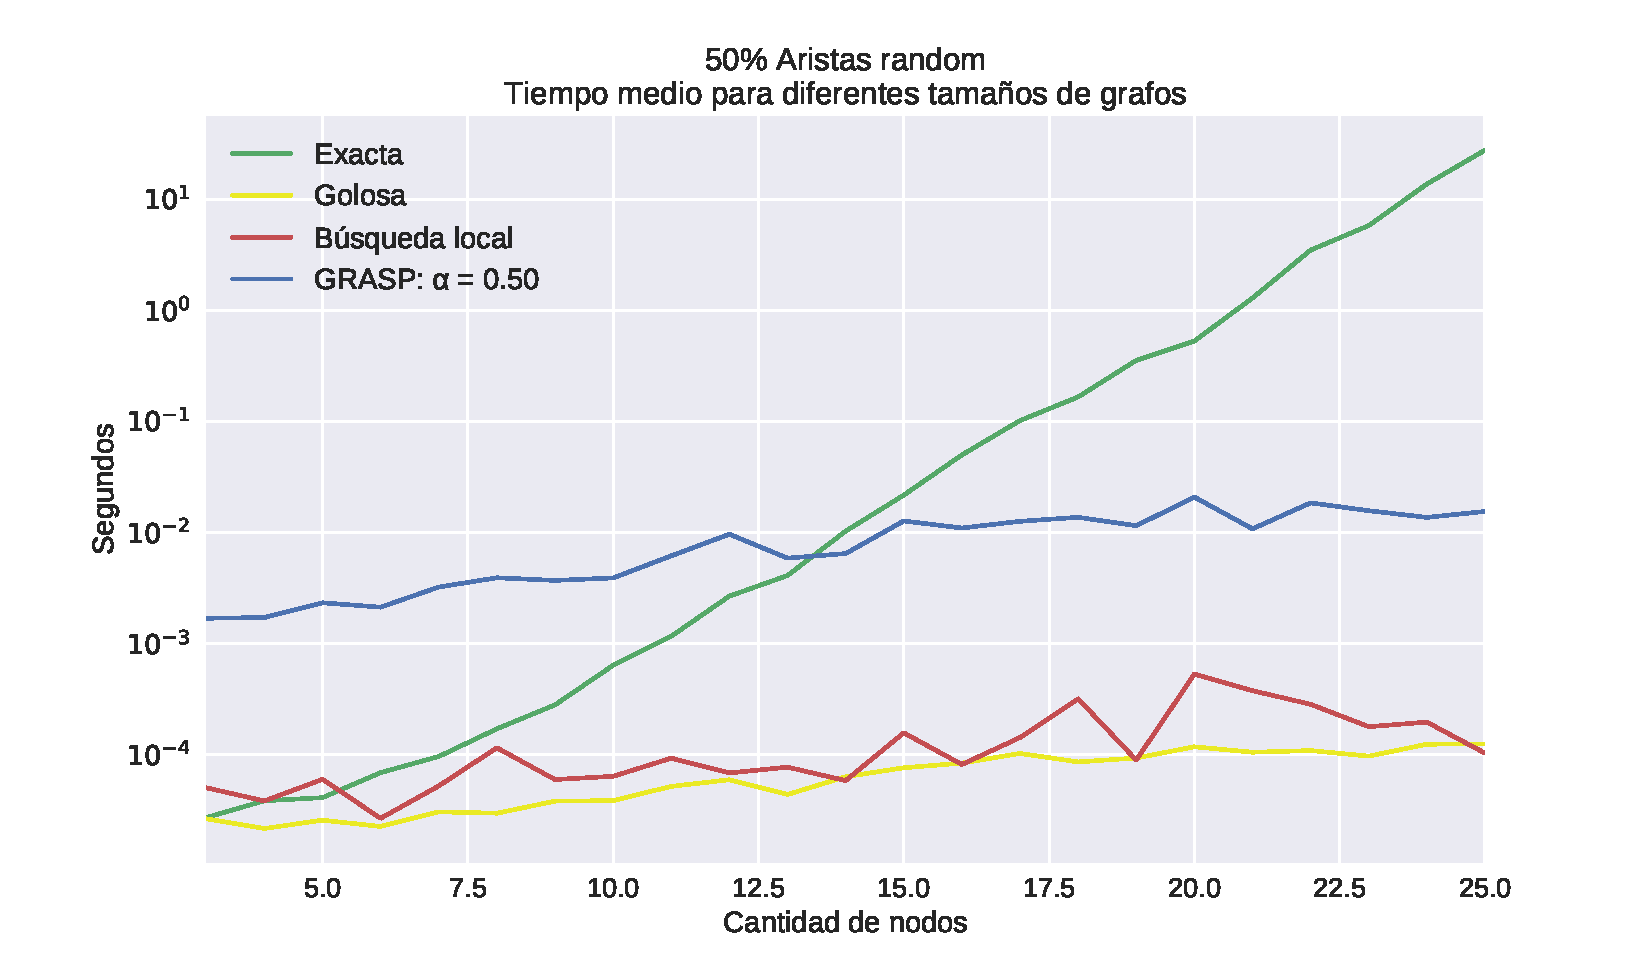
\includegraphics[width=1\textwidth]{informe/imgs/exp_random50_tiempo_todos_v2.pdf}
    \captionof{figure}{$\uparrow$ Escala logarítmica}
}

{\centering
    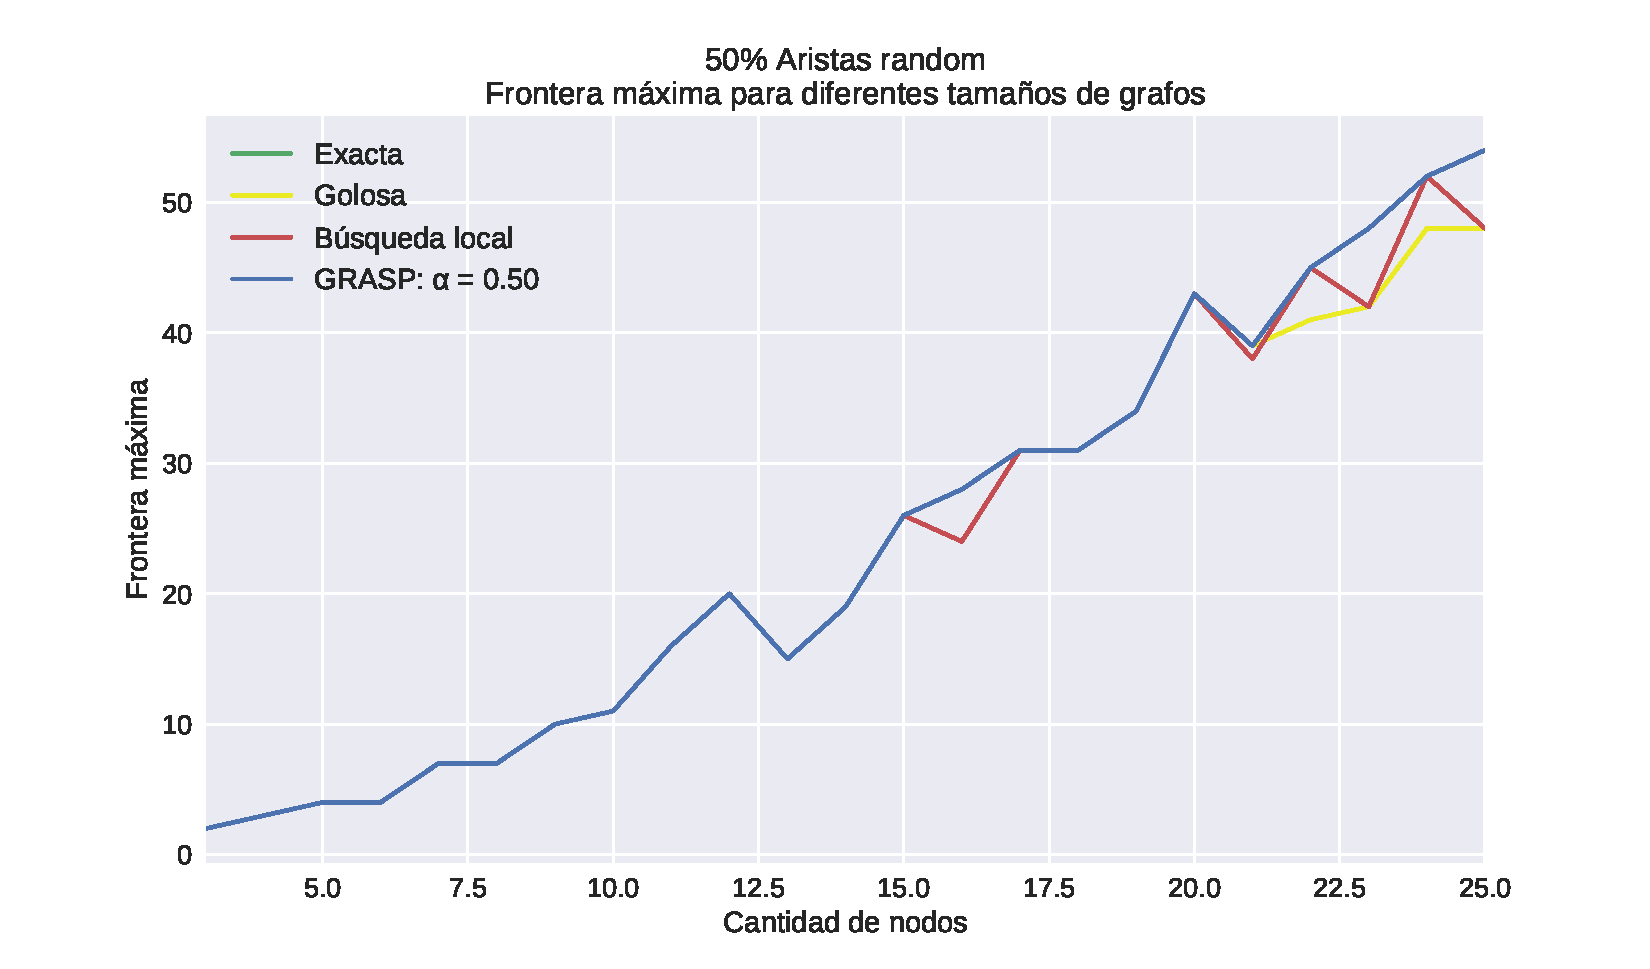
\includegraphics[width=1\textwidth]{informe/imgs/exp_random50_frontera_todos_v2.pdf}
}

{\centering
    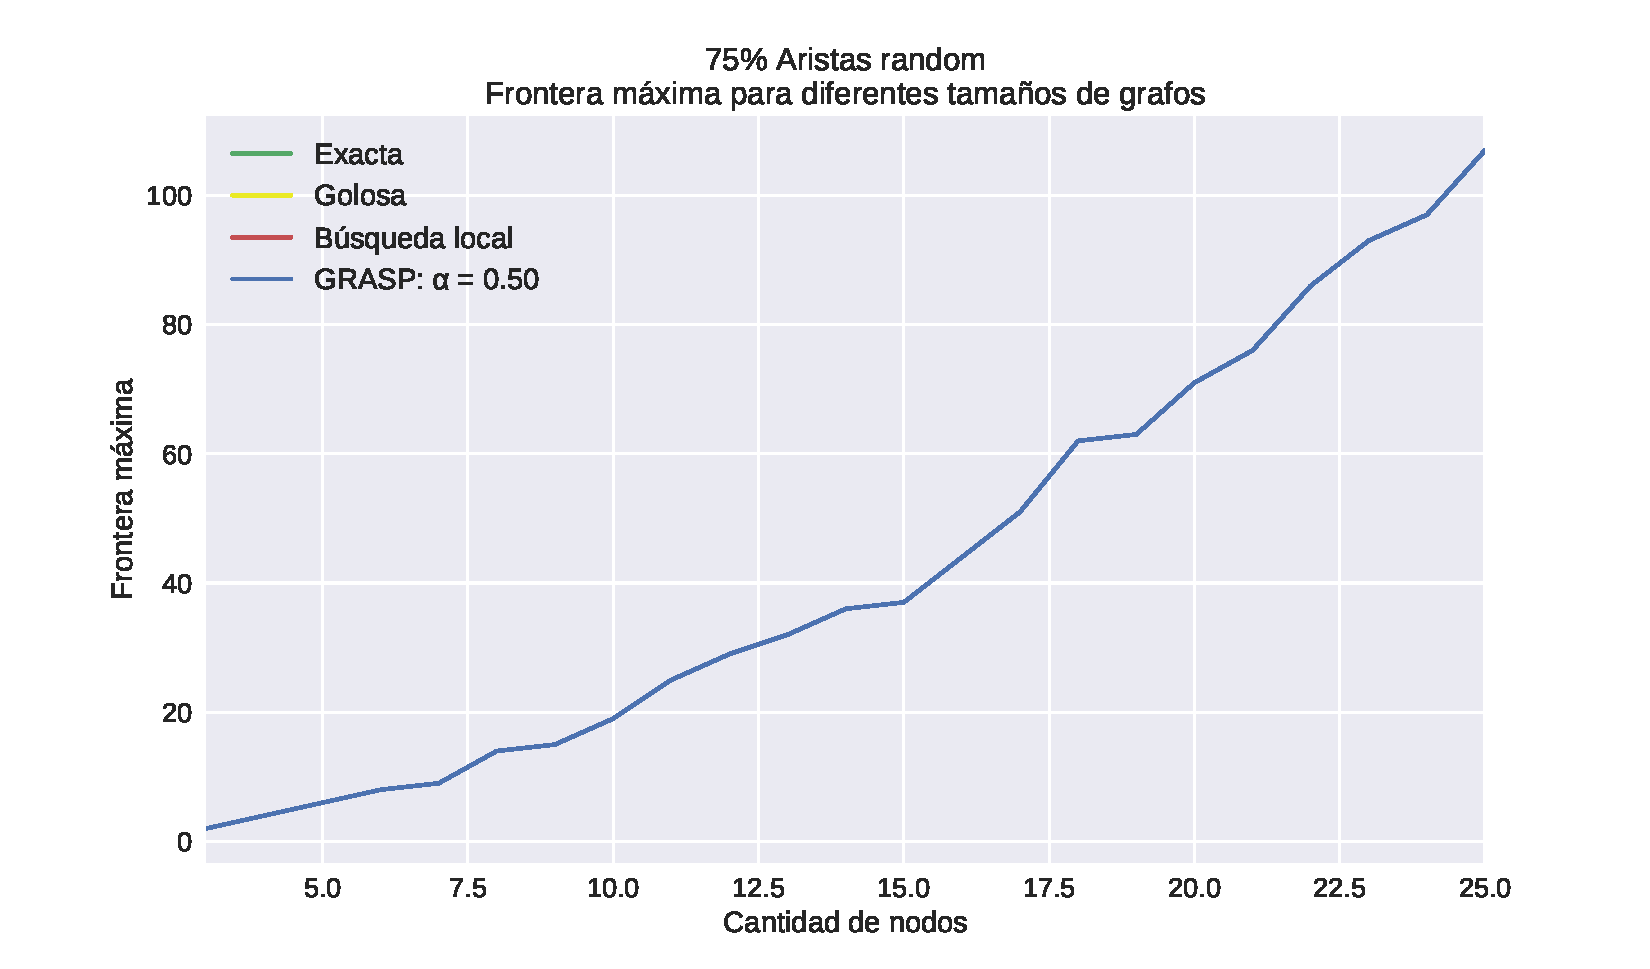
\includegraphics[width=1\textwidth]{informe/imgs/exp_random75_frontera_todos_v2.pdf}
}
